\section{\textcolor{red}{System Architecture/Experimental Setup}}
\label{section:system_architecture}

The work described in this dissertation is part of the AUGMANITY project\footnote{AUGMANITY website: \url{https://www.augmanity.pt}} that aims to develop technologies to support people operating in industrial environments. The experimental setup comprises the integration of both hardware and software components in a prototype collaborative cell (LARCC) at the Laboratory for Automation and Robotics (LAR) located in the Department of Mechanical Engineering at the University of Aveiro, as illustrated in \autoref{fig:LARCC}. The LARCC is equipped with a UR10e collaborative robot and multimodal sensor devices, including three LiDAR Velodyne sensors and four Orbbec 3D cameras distributed throughout the work volume. The software architecture is built upon the ROS middleware \cite{Quigley2009}, providing a robust framework for communication and coordination among the various components. In this context, this section provides a description of the materials used during this study and the methodological approaches followed to face the key challenges. 

\begin{figure}[ht]
    \centering
    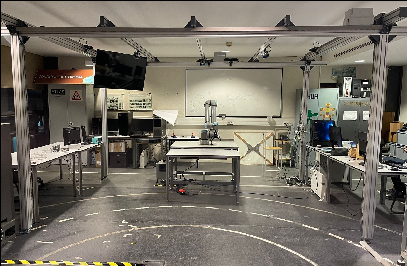
\includegraphics[width=0.75\columnwidth]{figs/LARCC_prototype.pdf}
    \caption{Prototype collaborative cell LARCC}
    \label{fig:LARCC}
\end{figure}

\if{0}
\begin{figure}[!ht]
\centerline{\includegraphics[width=0.9\textwidth, trim={0 5cm 0 0}, clip]{figs/setup2.jpg}}
\caption[setup]{LAR hardware setup}
\label{fig:LARCC}
\end{figure}
\fi

\subsection{Robot Operating System (ROS)}

ROS\cite{ROS2}\footnote{ROS 1 documentation: \url{https://wiki.ros.org}}\footnote{ROS 2 documentation: \url{https://docs.ros.org/en/humble}} is an open-source collection of tools and software libraries used to develop a robotics application and, in this work, it is used to establish communication throughout all of the infrastructure. ROS was chosen due to the hardware abstraction it offers given that it contains driver packages to deal with some hardware devices, allowing for easier communication with the robot and the cameras. Other relevant features include:
\begin{itemize}
    \item \textbf{message broker}: every process in the project is a node in the ROS network and communicates with the other nodes mainly through topics (asynchronous publish/subscribe streaming of data) or services (synchronous RPC-style communication).
    \item \textbf{code reuse}: executables and packages are written to be as independent as possible, making the developer able to reuse them in another project.
    \item \textbf{rich ecosystem}: there are several open-source packages available to the developer that can be easily integrated.
    \item \textbf{scalability}: given that the nodes are so loosely coupled, it allows for node distribution.
    \item \textbf{language independence}: nodes can be written in any language since communication is established through well-defined objects.
    \item \textbf{data visualization}: there are tools to visualize the data and the functioning of the system in real-time, such as Rviz.
    \item \textbf{simulator support}: ROS has support for simulators with Gazebo being the most common.
\end{itemize}

For this system, the ROS 1 Noetic distribution was chosen over the more recent ROS 2 distributions so as to take advantage of work already done by other members of the AUGMANITY project at the University of Aveiro.

\subsection{Perception System}
\label{subsection:perception_system}

In order to capture the necessary information from the environment, two Orbbec Astra Pro RGBD cameras were used. This camera model was developed by Orbbec Technologies and it is frequently used in computer vision and robotics \cite{AstraPro}. Among the available cameras, it was chosen since it allowed to capture both color and depth images.

\begin{figure}[ht]
\centerline{\includegraphics[width=0.6\textwidth]{figs/AstraPro.jpg}}
\caption[Orbbec Astra Pro]{Orbbec Astra Pro \cite{AstraPro}}
\label{fig:orbbec_astra_pro}
\end{figure}

In the experimental setup, one of the cameras is placed above the workspace facing downwards allowing the perception of the objects in the table through the color image and the position of the user through the depth image. The second camera is above and slightly behind the robot to capture the user in front of the robot with the images from this camera being the ones used in the keypoint detection models. The communication with the cameras is established through ROS with the $usb\_cam$ package being used for the color image and the $ros\_astra\_camera$ package being used for the depth image. In order to have better control over the lightness in the environment, only artificial lighting was used and the back-light compensation was raised to the maximum in the $usb\_cam$ configurations. Then the frame rate was also set to 10 frames per second in both cameras given that none of the following image processing tasks require a high frame rate.

As said before, the color image of the first camera is used to detect objects in the environment. These objects are blocks of specific colors and therefore they can be identified with color segmentation, which is done with the help of OpenCV\footnote{OpenCV documentation: \url{https://docs.opencv.org/4.x/}}, a popular computer vision library. With this library, the image from the camera is initially cropped to a specific region of interest consisting of the table area, which is then converted from BGR to HSV given that the intervals of a color are more reliable in this representation. From the HSV image and the color intervals, a mask is obtained for each color. These masks are then subject to a closing morphological operation to reduce any possible noise. Finally, the resulting areas are considered an object if they surpass a certain area threshold further reducing noise.

On the other hand, the depth image is used to obtain the position of the human in the workspace by cropping it to a certain region of interest corresponding to where the user would normally be and then detecting the highest point.

\subsection{Manipulator Arm Control}
\label{subsection:manipulator_arm_control}

The collaborative robot available for this work is a UR10e model which was developed by Universal Robots. This model has six degrees of freedom with six rotational joints, allows for payloads up to \SI{12.5}{\kilogram}, and has a reach of \SI{1300}{\milli\metre} being suitable for tasks such as machine tending, palletizing, and packaging\cite{UR10e}. In this work, the robot is equipped with a 2F-140 gripper developed by Robotiq, commonly used together with robot models from Universal Robots\cite{robotiq_gripper}.

\begin{figure}[ht]
    \centerline{\includegraphics[width=0.4\textwidth]{figs/UR10e.jpg} \ \ \includegraphics[width=0.35\textwidth]{figs/robotiq-2f-140.jpg}}
    \caption[UR10e Collaborative Robot and Robotiq 2F-140 Gripper]{UR10e Collaborative Robot \cite{UR10e_image} and Robotiq 2F-140 Gripper \cite{robotiq_gripper}}
    \label{fig:ur10e}
\end{figure}

Both the robot and the gripper have ROS packages containing their drivers making their integration easier. The planning and execution of the arm movements are done through the MoveIt\footnote{MoveIt documentation: \url{https://ros-planning.github.io/moveit_tutorials}} framework, which is a widely-used open-source framework for robotics applications involving motion planning, manipulation, 3D perception, kinematics, control, navigation, and collision checking, with OMPL being chosen to handle the motion planning tasks.

The configurations of the drivers and MoveIt was already done by other members of the AUGMANITY project and can be found on Github\footnote{Github LarCC Repository: \url{https://github.com/afonsocastro/larcc_interface}} along with a higher-level API that encloses that logic. During this work, an additional feature to stop movements was added.

\subsection{Computational Systems}

The tasks involved in this work, such as training deep-learning models and analyzing images in real-time require high computational resources. To handle the real-time processing of images and robot control, the central computer present in the setup was used. To handle the deep-learning model training, the deep-learning research server from LAR was used, codenamed Deeplar:
\begin{itemize}
    \item AMD RyzenTM Threadripper 2950X;
    \item Four NVIDIA GEFORCE® RTX 2080 Ti;
    \item 128GB DDR4 RAM.
\end{itemize}

The model training in Deeplar is executed using docker images, which allows multiple people to use the computer with each having their own isolated training environment with their own dependencies. The images used to design and train machine learning models in this work are based on the latest TensorFlow official image for GPUs.

TensorFlow is one of the most popular machine learning frameworks along with Pytorch. In this work, the former was chosen over the latter since the higher-level API allowed for faster development. The main features of Tensorflow\footnote{Tensorflow documentation: \url{https://www.tensorflow.org/api_docs}} are:
\begin{itemize}
    \item \textbf{prepare data}: load data, data pre-processing and data augmentation;
    \item \textbf{build models}: design and train custom models with little code or use pre-trained ones (transfer learning);
    \item \textbf{deploy models}: helps using models in different platforms such as locally, in the cloud, in a browser, or in mobile;
    \item \textbf{implement MLOps}: run models in production, tracking their performance and identifying issues.
\end{itemize}

\subsection{Keypoints Detection}
\label{subsection:keypointdetection}

MediaPipe\footnote{MediaPipe documentation: \url{https://developers.google.com/mediapipe}} consists of a set of libraries and tools to apply AI and Machine Learning techniques in other applications, particularly in pipelines for advanced real-time vision-based applications \cite{Lugaresi2019}. Although it contains many features, in this work the focus is on the Hand and the Pose Landmark Detection Models.
The Hand Landmark Detection model \cite{Zhang2020} uses two sub-modules: a hand palm detection model and a hand landmark model. Each frame of an RGB input is fed into the palm detection model, which produces a bounding box based on the palm. The hand landmark model uses this bounding box and returns the keypoint localization of 21 landmarks, including the fingertips, the finger joints (knuckles), and the base of the palm (\autoref{fig:mediapipe_hand_landmarks}). The Pose Landmark Detection model also uses two sub-modules working in a similar way to return 33 landmarks over the entire body (\autoref{fig:mediapipe_pose_landmarks}).

\begin{figure}[ht]
    \centering
    \begin{subfigure}[b]{0.49\textwidth}
        \adjincludegraphics[width=\textwidth, trim={{.15\width} {0} {.05\width} {0}}, clip]{figs/hand_landmarker.jpg}
        \caption{}
        \label{fig:mediapipe_hand_landmarks}
    \end{subfigure} \
    \begin{subfigure}[b]{0.49\textwidth}
        \adjincludegraphics[width=\textwidth, trim={{0} {0} {.20\width} {0}}, clip]{figs/pose_landmarker.jpg}
        \caption{}
        \label{fig:mediapipe_pose_landmarks}
    \end{subfigure}
    \caption[Mediapipe landmarker models: Hand Landmarker and Pose Landmarker.]{Mediapipe landmarker models \cite{mediapipe_docs}: (a) Hand Landmarker and (b) Pose Landmarker.}
    \label{fig:mediapipe_landmarks}
\end{figure}

\subsection{RL Simulator}

\textcolor{red}{Gymnasium and Mujoco}